%% Submissions for peer-review must enable line-numbering 
%% using the lineno option in the \documentclass command.
%%
%% Preprints and camera-ready submissions do not need 
%% line numbers, and should have this option removed.
%%
%% Please note that the line numbering option requires
%% version 1.1 or newer of the wlpeerj.cls file, and
%% the corresponding author info requires v1.2

\documentclass[fleqn,10pt,lineno]{wlpeerj} % for journal submissions
% \documentclass[fleqn,10pt]{wlpeerj} % for preprint submissions

\title{Comparison of large-scale citizen science data and long-term study data for phenology modeling}

\author[1]{Shawn D. Taylor}
\author[2]{Joan M. Meiners}
\author[3]{Kristina Riemer}
\author[4]{Michael C. Orr}
\author[5]{Ethan P. White}

\affil[1,2]{UFL SNRE}
\affil[4]{Key Laboratory of Zoological Systematics and Evolution, Institute of Zoology, Chinese Academy of Sciences, Beijing 100101, P.R. China}
\affil[3,5]{UFL WEC}
\affil[5]{UFL Bioinformatics}
\corrauthor[1]{Shawn D. Taylor}{shawntaylor@weecology.org}

% \keywords{Keyword1, Keyword2, Keyword3}

\begin{abstract}
\end{abstract}

\begin{document}

\flushbottom
\maketitle
\thispagestyle{empty}

\section*{Introduction}

Robust plant phenology models are necessary for forecasting the future state of the ecological systems at several scales, from global climate to impacts on plant and animal communities. Plant phenology performs an important role in many fields of ecological research such as ecosystem function, carbon dynamics, pollination, and community ecology \citep{richardson2013, cleland2007, tang2016}. At the largest scale, variation in the timing of spring leaf out and fall senescence account for a significant amount of uncertainty in the carbon budget of earth system models, which has implications for correctly accounting for biosphere-atmosphere feedbacks in long-term forecasts \citep{richardson2012}. At local scales, because of species specific responses to temperature and precipitation, changes in flowering times can alter the flower community throughout the growing season \citep{caradonna2014, diez2012, theobald2017}. This change in resource availability can affect the abundance and richness of pollinators \citep{ogilvie2017a, ogilvie2017b}, and higher trophic levels \citep{tylianakis2008}. Accurately accounting for phenology in these and other scenarios will be critical for forecasting environmental change.  

To best forecast plant phenology researchers will need models which account for the full range of variation across a species range \citep{richardson2013, chuine2017}. Many plant phenological studies in the past have relied upon datasets collected at a single location over a long time-frame by a single group \citep{cook2012, roberts2015, iler2013, wolkovich2012}. These datasets have high temporal coverage, with some approaching several decades, and represent the species and climate variability at their respective sites extremely well. Yet it is common for phenology models built with observations from a single site to not transfer well to other sites \citep{garcia-mozo2008, xu2013, olsson2014, basler2016}. This lack of transferability across space can be driven by, among other factors, plasticity in phenology requirements, local adaptation, microclimates, plant age, or population density \citep{kramer1995, diez2012}. Future models which account for this variability will require data from as much of a species' range as possible. Further, data from a single location may not be adequate for ecosystem level phenology modelling due to a potentially limited species pool. Thus, new sources of data beyond traditional single site studies will be needed.

Citizen science data is becoming increasingly important for ecological research, with the potential for significant impact in many fields \citep{dickinson2010, tulloch2013, kelling2009}. Citizen science efforts have helped document range shifts \citep{hitch2007}, study the effect of landscape fragmentation on amphibians \citep{cosentino2014}, and informed ecological theory of community composition \citep{locey2013}. A relatively new citizen science group, The National Phenology Network (NPN) is an organization which accepts phenology observations from volunteers throughout North America and makes the data freely available \citep{schwartz2012a}. The NPN dataset has already been used to study, among many things, variation in oak phenology \citep{gerst2017}, large-scale community phenology models \citep{melaas2016}, and forecasting long-term phenology trends \citep{jeong2013}. The regional to continental scale of citizen science data helps researchers explain large-scale patterns across natural gradients, but can also introduce new sources of error from observer skill, variation in sampling effort, and spatial bias \citep{dickinson2010}. These issues can be accounted for in models but first must be identified and quantified. With hundreds of observers across North America, the observer and sampling bias for species identification and the true date of phenological events is potentially high. Though volunteers can be very accurate at distinguishing different phenophases \citep{fuccillo2015}, observations can still be made sporadically throughout the growing season, some years skipped, or visits to a particular site discontinued entirely. 

While there have been several studies looking at best practices when using the NPN dataset \citep{crimmins2017, gerst2016}, no study to date has compared it directly with data from long-term studies to test its adequacy for plant phenology models. Data from long-term studies (LTS) have been invaluable for phenology research for several decades, but datasets with a larger spatial extent and more complete species pools will be needed to model the complex phenological dynamics of ecosystems \citep{richardson2012, diez2012, caradonna2014}. Such datasets from China and Europe have already contributed considerably to phenological research \citep{olsson2014, basler2016, xu2013, zhang2017}, and the NPN dataset has the potential to meet these needs for North American plant species and communities. Here, we fit seven different plant phenology models to the budburst and first flowering phenophases of XX plant species. The models were fit twice, once using data from the NPN dataset, and again for the same species using data from an LTS dataset. We then compared three outputs between the two sets of models built using NPN and LTS data: 1) the models' parameter estimates; 2) the models' estimates of phenophase timing; and 3) the models' errors using held out testing data.

\section*{Methods}

\subsection*{Datasets}

The National Phenology Network observations are based on status-based monitoring, where observers answer yes, no, or unsure when asked if an individual plant has a specific phenophase present \citep{denny2014}. Phenophases refer to specific phases in the annual cycle of a plant, such as the presence of emerging leaves, flowers, fruit, or senescing leaves. We downloaded all NPN observations from 2009, when collections began, to 2016 for the phenophases Breaking Leaf Buds, Breaking Needle Buds, Emerging Needles, and Open Flowers. The first three phenophases apply to the leaf out phase for deciduous broadleafs, evergreen conifers, and pines, respectively. The Open Flowers phenophase indicates fully open flowers and applies to all angiosperms. Hereafter we will refer to these as either Flowers for the Open Flower phenophase, or Budburst for all other phenophases. 

We used moderately strict subsetting of NPN phenology observations as outlined in \cite{crimmins2017}. First, "yes" observations for individual plants were only kept if they were preceded by a "no" observation within 30 days. Observations for Budburst past day of year (DOY) 172 and for Flowers past DOY 213 were dropped to minimize any influence from outliers. Finally, only species that had greater than 30 total observations were kept. \cite{crimmins2017} only kept observations that were preceded by a "no" within 15 days, and also grouped multiple individuals at single sites to a single observation. We used 30 days to allow for a greater number of species to be compared. We did not group together multiple individuals at a single site to better incorporate intra-site variability. In addition to these steps we also inferred the date of each phenophase as the midpoint between each "yes" observation and the preceding "no" observation. 

To compare against the NPN dataset we used four LTS datasets from North America (Table 1), representing three major ecosystem types and 24 species. Observation metrics varied among these four datasets due to different protocols, so were first converted to binary "yes" and "no" observations for each phenophase (see supplement for details). As with the NPN dataset, we infer the date for each phenophase as the midpoint between the first "yes" observation and most recent "no" observation. 

\renewcommand{\arraystretch}{2}\tabcolsep=5pt
\begin{center}
    \begin{tabular}{ | l | l | l | l |}
    \hline
    Dataset Name & Habitat &  Phenological Event\newline (Num. Species) & Reference \\ \hline
    Harvard & N.E. Deciduous\newline Forest & Budburst (16)\newline Flowering (15) & \citep{okeefe2000} \\
    Jornada & Chihuahuan Desert & Flowering (2) & ... \\
    HJ Andrews \newline Experimental Forest & N.W. Wet Coniferous \newline Forest & Budburst (6)\newline Flowering (6) & ... \\
    Hubbard Brook & N.E. Deciduous \newline Forest & Budburst (3) & ... \\
    \hline
    \end{tabular}
\end{center}

\subsection*{Models}

Plant species all have unique phenological requirements, thus it is common to fit several types of models to find the one which best represents a specific species \citep{chuine2013}. For each species/phenophase in each of the five datasets, we fit a range of phenology models from a naive mean day of year estimate to a more complex two phase forcing model (Table 2). The naive model uses only the mean DOY from all prior observations as the estimated DOY. The linear model uses a regression with the mean spring (Jan. 1 - March 31) temperature as the only independent variable and DOY as the response variable.

For the remaining models the general form form predicts that a phenological event will happen when sufficient thermal forcing units, $F^{*}$, accumulate from a particular start day of the year ($t_{1}$). The start day can either be estimated or fixed. For the growing degree day model (GDD) forcing units are the total degrees above the threshold $T$. The Fixed GDD model uses the same form but has fixed values for start day ($t_{1}$ = Jan 1) and temperature threshold ( $T$ = 0C). The Alternating model has a variable number of required forcing units defined as a function of the total number of days below 0C since Jan. 1 ($NCD$). The Uniforc model is similar to the GDD model but has forcing units transformed via a sigmoid function \citep{chuine2000}.

Finally, two models attempt to explain the spatial variation in phenological requirements. The first spatial model, M1, is an extension of the GDD model which adds a correction in the required forcing using the photoperiod ($L$) \citep{blumel2012}. The second, the Macroscale Species-specific Budburst model (MSB), uses the mean spring temperature as a linear correction on the total forcing required in the Alternating model \citep{jeong2013}. Since there is little to no spatial variation in the LTS datasets, the two spatial models were fit using only the NPN dataset. The resulting parameters, estimates, and errors for the NPN derived M1 and MSB models were compared to the LTS GDD and Alternating models, respectively, for each species and phenophase.  

\begin{center}
{\def\arraystretch{2}\tabcolsep=5pt
    \begin{tabular}{ | l | c | c | p{1.3cm} | l |}
    \hline
    Name & DOY Estimator & Forcing Equations & Total\newline Parameters & Reference \\ \hline
    Naive & \( \overline{DOY} \) & - & 1 & - \\
    Fixed GDD &$\sum_{t=0}^{DOY}R_{f}(T_{i})\geq F^{*} $  & $R_{f}(T_{i}) = min(T_{i}, 0)$ & 1 & - \\
    Linear & \( DOY = \beta_{1} + \beta_{2}T_{mean} \) & - & 2 & - \\
    GDD & $\sum_{t=t_{1}}^{DOY}R_{f}(T_{i})\geq F^{*} $ & $ R_{f}(T_{i}) = max(T_{i} - T^{*}, 0) $  & 3 & - \\
    M1 & $\sum_{t=t_{1}}^{DOY}R_{f}(T_{i})\geq (\frac{L_{i}}{24})^{k} F^{*} $ & $ R_{f}(T_{i}) = max(T_{i}-T^{*}, 5) $  & 4 & \citep{blumel2012} \\
    Alternating & $\sum_{t=0}^{DOY}R_{f}(T_{i})\geq a + be^{cNCD(t)} $ & $R_{f}(T_{i}) = max(T_{i}-5, 0) $ & 3 & \citep{cannell1983} \\
    MSB & $\sum_{t=0}^{DOY}R_{f}(T_{i})\geq a + be^{cNCD_{i}} +dT_{mean} $ & $R_{f}(T_{i}) = max(T_{i}-5, 0) $ & 4 & \citep{jeong2013} \\
    Uniforc &  $\sum_{t=t_{1}}^{DOY}R_{f}(T_{i})\geq F^{*} $ & $ R_{f}(T_{i}) = \frac{1}{1 + e^{b(T_{i}-c)}} $ & 4 & \citep{chuine2000} \\

    \hline
    \end{tabular}
    }
\end{center}

All models were parameterized using differential evolution to minimize the root mean square error (RMSE) of the estimated day of year of the phenological event. Differential evolution is a global optimization algorithm which uses a population of randomly initialized models which converge set of parameters which minimize the RMSE \citep{storn1997}. Confidence intervals for parameters were obtained by bootstrapping, where individual models were re-fit 250 times using a random sample, with replacement, of the data. A random 20\% of all data was held out from model fitting for use in later evaluation. Predictions were made by taking the mean DOY from the 250 bootstrapped models. 

\subsection*{Analysis}

As described above, two sets of models were produced for each species and phenophase: one set of models parameterized using only NPN data, and one set parameterized using only LTS data (with the exception of the M1 and MSB models, see above). The distribution for each parameter in each species/phenophase model was compared between the two sets (LTS and NPN) using a Mann-Whitney test. This was chosen due to the majority of parameters having non-normal distributions. Using the mean value of each bootstrapped parameter we also calculated the coefficient of determination ($R^2$) between LTS and NPN derived models among the 39 species-phenophases. 

Even models with different parameter values, even entirely different model structure, can still produce similar estimates for the date of phenological events \citep{basler2016}. Thus, we also compared the estimated DOY between LTS and NPN derived models. For estimates made at the four LTS sites, across all NPN sites, and for each of the 6 models we calculated the coefficient of determination ($R^2$) between LTS and NPN derived estimates.   

To evaluate model performance we outlined four scenarios: A) LTS derived models used to predict LTS observations, B) NPN derived models used to predict LTS observations, C) LTS derived models used to predict NPN observations, and D) NPN derived models used to predict NPN observations. Within each of these scenarios we calculated the RMSE of the held out observations for each species, phenophase, and  model type. Due to varying sample sizes the RMSE values cannot be easily compared directly, thus we calculated two simple difference metrics for the relative performance of LTS and NPN derived models. Using RMSE values from the four scenarios metric 1, $RMSE_{A} - RMSE_{B}$ , compared models at the four LTS sites and metric 2, $RMSE_{C} - RMSE_{D}$, compares models at all NPN sites, representing a large spatial scale. In both metrics negative values indicate LTS derived models perform better while positive values indicate the NPN derived model performed better. Absolute RMSE values are provided in the supplement (Fig. S1-S3).


\begin{figure}[]
	\centering
		\includegraphics[width=1\textwidth]{fig_1_param_comparison.png}
	\caption{Comparisons of parameters between NPN and LTS derived models. Each point represents a parameter value for a specific species/phenophase, and is the mean value from 250 bootstrapped  models. The black line is a 1:1 line, and $R^2$ is the coefficient of determination.}
\end{figure}


\section*{Results}

The Fixed GDD model, followed by the Linear model had the highest $R^2$ between parameters of NPN and LTS derived models, while parameters for all other models had $R^2$ values < 0 (Fig. 1). The variation around each parameter was high and uneven between LTS and NPN derived models, as all parameters had statistically different (p < 0.001) distributions between NPN and LTS derived models according to the Mann-Whitney U test. The Naive model showed a distinct late bias in the mean DOY for phenological events, likely resulting from the LTS datasets being mostly in the northern United States. Though it still has a small bias, the Fixed GDD model had the best correlation ($R^2=0.49$ for the single parameter) between the two datasets. The outlier for this model, \textit{Larrea tridentata}, has phenology largely driven by precipitation, which is not considered in the Fixed GDD model \citep{beatley1974}. 

\begin{figure}
	\centering
		\includegraphics[width=1\textwidth]{fig_2_estimate_compare.png}
	\caption{Comparison of estimates between NPN and LTS derived models, made only at LTS sites (top panel) or among all NPN sites (bottom panel). Each point is a single observation. Different colors indicate observations for a single species/phenophase.}
\end{figure}

When comparing estimates of phenological events between the two sets of models, many NPN and LTS models produced similar estimates (Fig. 2). The Fixed GDD model had the highest correlation between the two models sets at NPN sites ($R^2 = 0.82$), while the GDD, M1, and Uniforc models had the highest correlation at LTS sites ($R^2 = 0.54$). The MSB (an extension of the alternating model which adds a spatial correction based on mean spring temperature, see Table 2 and methods) improved the correlation between the two datasets over the Alternating model. The MSB model improved the $R^2$ from 0.38 to 0.45 at LTS sites, and from -0.2 to -0.13 at NPN sites. The M1 model (an extension of the GDD model which adds a spatial correction based on daylength) did not improve the correlation between datasets over the GDD model. 

NPN derived models perform better predicting held out NPN observations, while LTS derived models perform better predicting held out LTS observations (Fig. 3). The Naive and Linear models had the largest differences between the two model sets, while the Fixed GDD model had relatively similar errors when evaluated on both NPN and LTS held out observations. Though the Fixed GDD model had the highest agreement in errors between NPN and LTS derived models, it was not the best performing model overall. The GDD and Uniforc were commonly the most best performing, having the lowest RMSE in 22\% and 40\% of cases among NPN derived models, and 42\% and 32\% of cases among LTS derived models, respectively (Fig. S1 & S2).


\begin{figure}
	\centering
		\includegraphics[width=1\textwidth]{rmse_metrics_density_plot.png}
	\caption{Density plots for the two different metrics. Each plot represents the metric value for the 39 species/phenophase comparisons. The metric represents the difference in RMSE values between the difference scenarios (A - B, or C - D).}
\end{figure}


\section*{Discussion}

\subsection{Discussion intro}

Here we compared two datasets which are typical in ecology. One is intensively studied with a long time series from several locations, the other has a large spatial coverage of hundreds of locations, but with no single location having a long timeseries. We show that they vary in parameter estimates and observation estimates in all but the simplest models, and regardless of the model they each predict their own out of sample data better than the other. Uses of each type of dataset thus depends on the desired research goals. Analyzing trends in response to changing climate will likely require using a long term study dataset, but extrapolation of those results to other locations must be done with care. Studying floral resource availability across a spatial gradient would be best done with NPN as it has a large number of species available, but attributing 

Here we emphasize the goal of large scale forecasting, where models must be built to the best estimate of the desired event, they must have independent/predictor variables which are currently available or forecastable (ie. temperature), and they must be able to extrapolate to new locations with no prior observations. While models built using the LTS datasets are able to give the best estimates for their locations, they do not perform better than NPN models on large scale data. This decrease in model performance with distance in single site phenology models is well known \citep{basler2016, xu2013, garcia-mozo2008}. 

The NPN dataset will be ideal in making large scale forecasts, but the ideal situation will be to integrate all types of data into analysis and forecasts. Datasets which have a long time series contain valuable information on the inter annual variation, the PHENOCAM network has a large spatial extent as well as fine temporal grain \citep{richardson2018}, and phenology derived from satellite imagery has worldwide coverage. Here straightforward models require all data to be from the same source, and give equal weight to all observations. More complex data integration methods can use data from all different sources to give the best estimate for forecasts \citep{ogle2015} and continuously update forecasts as new real time data becomes available \citep{luo2011}. 

\subsection{Details of the differences seen in the analysis}

Despite having statistically different parameters to LTS derived models, many NPN derived models were able to produce similar estimates for phenological events when using a single parameter Fixed GDD model. This is likely due to models being non-identifiable. For example, two GDD models with parameters of $t_{1}$=1, $F$=10, $T*$=0 and $t_{1}$=5, $F$=5, $T*$=0 can produce nearly identical results in many, but not all, scenarios. This makes the interpretation of these parameters difficult, which is troublesome as they are designed to be biologically relevant. For example the total forcing required, $F^*$, reflects the amount of heating in the spring required for a phenological even to occur. Here we show that there is little agreement when these parameters are estimated for the same species using two datasets. 

\cite{chuine2016} found similar issues, where models estimating endodormancy break using only observed budbreak did not match direct measurements of endodormancy break, suggesting that phenology models which are fit using only the observed phenophase cannot accurately infer the internal mechanisms described in the models. \cite{basler2016} suggests that the thermal forcing in models is responsible for most of the accuracy, while any additional parameters are only fit to residuals and sensitive to over fitting. Here, our simplest model, the Fixed GDD model which uses only a warming component, had the highest correlation of it's single parameter between LTS and NPN datasets. This correlation decreases as more parameters are added to models, suggesting that if the NPN dataset is being used to make inferences about plant physiology, simple models could give more consistent results. Parameter estimates of more complex models do not agree with models from the same species in LTS datasets, and it is possible even the LTS datasets are over fitting these models. 

One goal of ecological forecasting is to inform decision makers about the future state of systems \citep{dietz2018}. Thus, the best performing model should be used in these cases to give the best possible forecast. In terms of lowest RMSE the GDD and Uniforc The GDD and Uniforc models show promise for building models with the NPN dataset and making plant phenology forecasts across large scales as they were the best performing models for the majority of species and phenophases (fig. S1). Even with similar parameters, the Fixed GDD model was not the best performing model when tested on held out data. While the values of additional parameters may be incorrect in the sense of the prior paragraph, they nonetheless provide more predictive power. 

Other models show promise for forecasting under different scenarios. For example, if using data from a large spatial extent to make predictions at single sites (sensu. Scenario B) our results show that the Alternating model is the best option, as performance under this scenario is very similar to performance of Alternating models built from LTS data (Fig. 3). In the opposite scenario of making large-scale predictions using only data from a single site (sensu. Scenario C) the Fixed GDD model is likely the best option, as most LTS derived Fixed GDD models have a RMSE only 5 days greater, on average, than the corresponding NPN model (Fig. 4). The Alternating model is also one of the best performing model overall for large-scale NPN data (Fig. 3a). 

The models which incorporate a spatial component did not improve over their base models. Correspondence between parameter estimates (Fig. 1), estimates of phenological events (Fig. 2), and out of sample error rates (Fig. 3 & 4) for the MSB and M1 models were essentially the same as the Alternating and GDD models, respectively. The MSB and M1 models had the lowest error in 9 out of 39 occasions, but never by more than a single day over other models (Fig S1). Spatial variation in phenological requirements is known to exist in plants \citep{zhang2017}, yet here models which attempt to account for this variation did not improve estimates overall. This could be caused either by models not adequately capturing the process driving the spatial variation, the NPN dataset having biases from variation in sampling effort and/or spatial auto-correlation, or some combination of these factors. \cite{basler2016} used the M1 model to predict budburst on six species across Europe and found it was usually among the best models in terms of RMSE, albeit never by more than a single day. Their result was strengthened by a 40 year timeseries across a large region. \cite{chuine2017} noted that incorporating the spatial variation in warming requirements as a key issue in future phenology research. We feel the NPN dataset, as well as other large-scale phenology datasets, will be key in addressing this and other phenological research needs. 

\section*{Conclusion}

Currently the best phenology model for a single location will be one fit using data from only that location, yet these single site models do not transfer well to large scales. Making large-scale phenology forecasts will require the incorporation of large-scale observations such as those from the NPN dataset. Here we have shown that the NPN dataset is capable of parameterizing phenology models which make comparable predictions to LTS datasets. Indeed, if making forecasts across a large spatial extent the NPN derived models are preferable to LTS derived models. If using the NPN dataset to make inferences about plant physiology researchers should not use overly complicated models, as parameter estimates from complex NPN derived models do not agree with LTS derived models. Whether this disagreement stems from the spatial variation in plant phenology requirements, the irregular sampling of the NPN dataset, or the non-identifiability of models is an avenue for future study. 

The National Phenology Network dataset will likely be an important resource for studying phenology. The addition of numerous species and observations from across a range of conditions is important for informing large-scale processes, as similar datasets have shown in Europe \citep{olsson2014, basler2016} and Asia \citep{xu2013, zhang2017}. Research from long-term small scale studies has been invaluable and should no doubt be continued, but can now be complimented by using large-scale NPN data (ie. \citep{jeong2013, melaas2016}).

\section*{Acknowledgments}

\bibliography{refs}

\setcounter{figure}{0}    
\section*{Supplement}
\begin{figure}
	\centering
		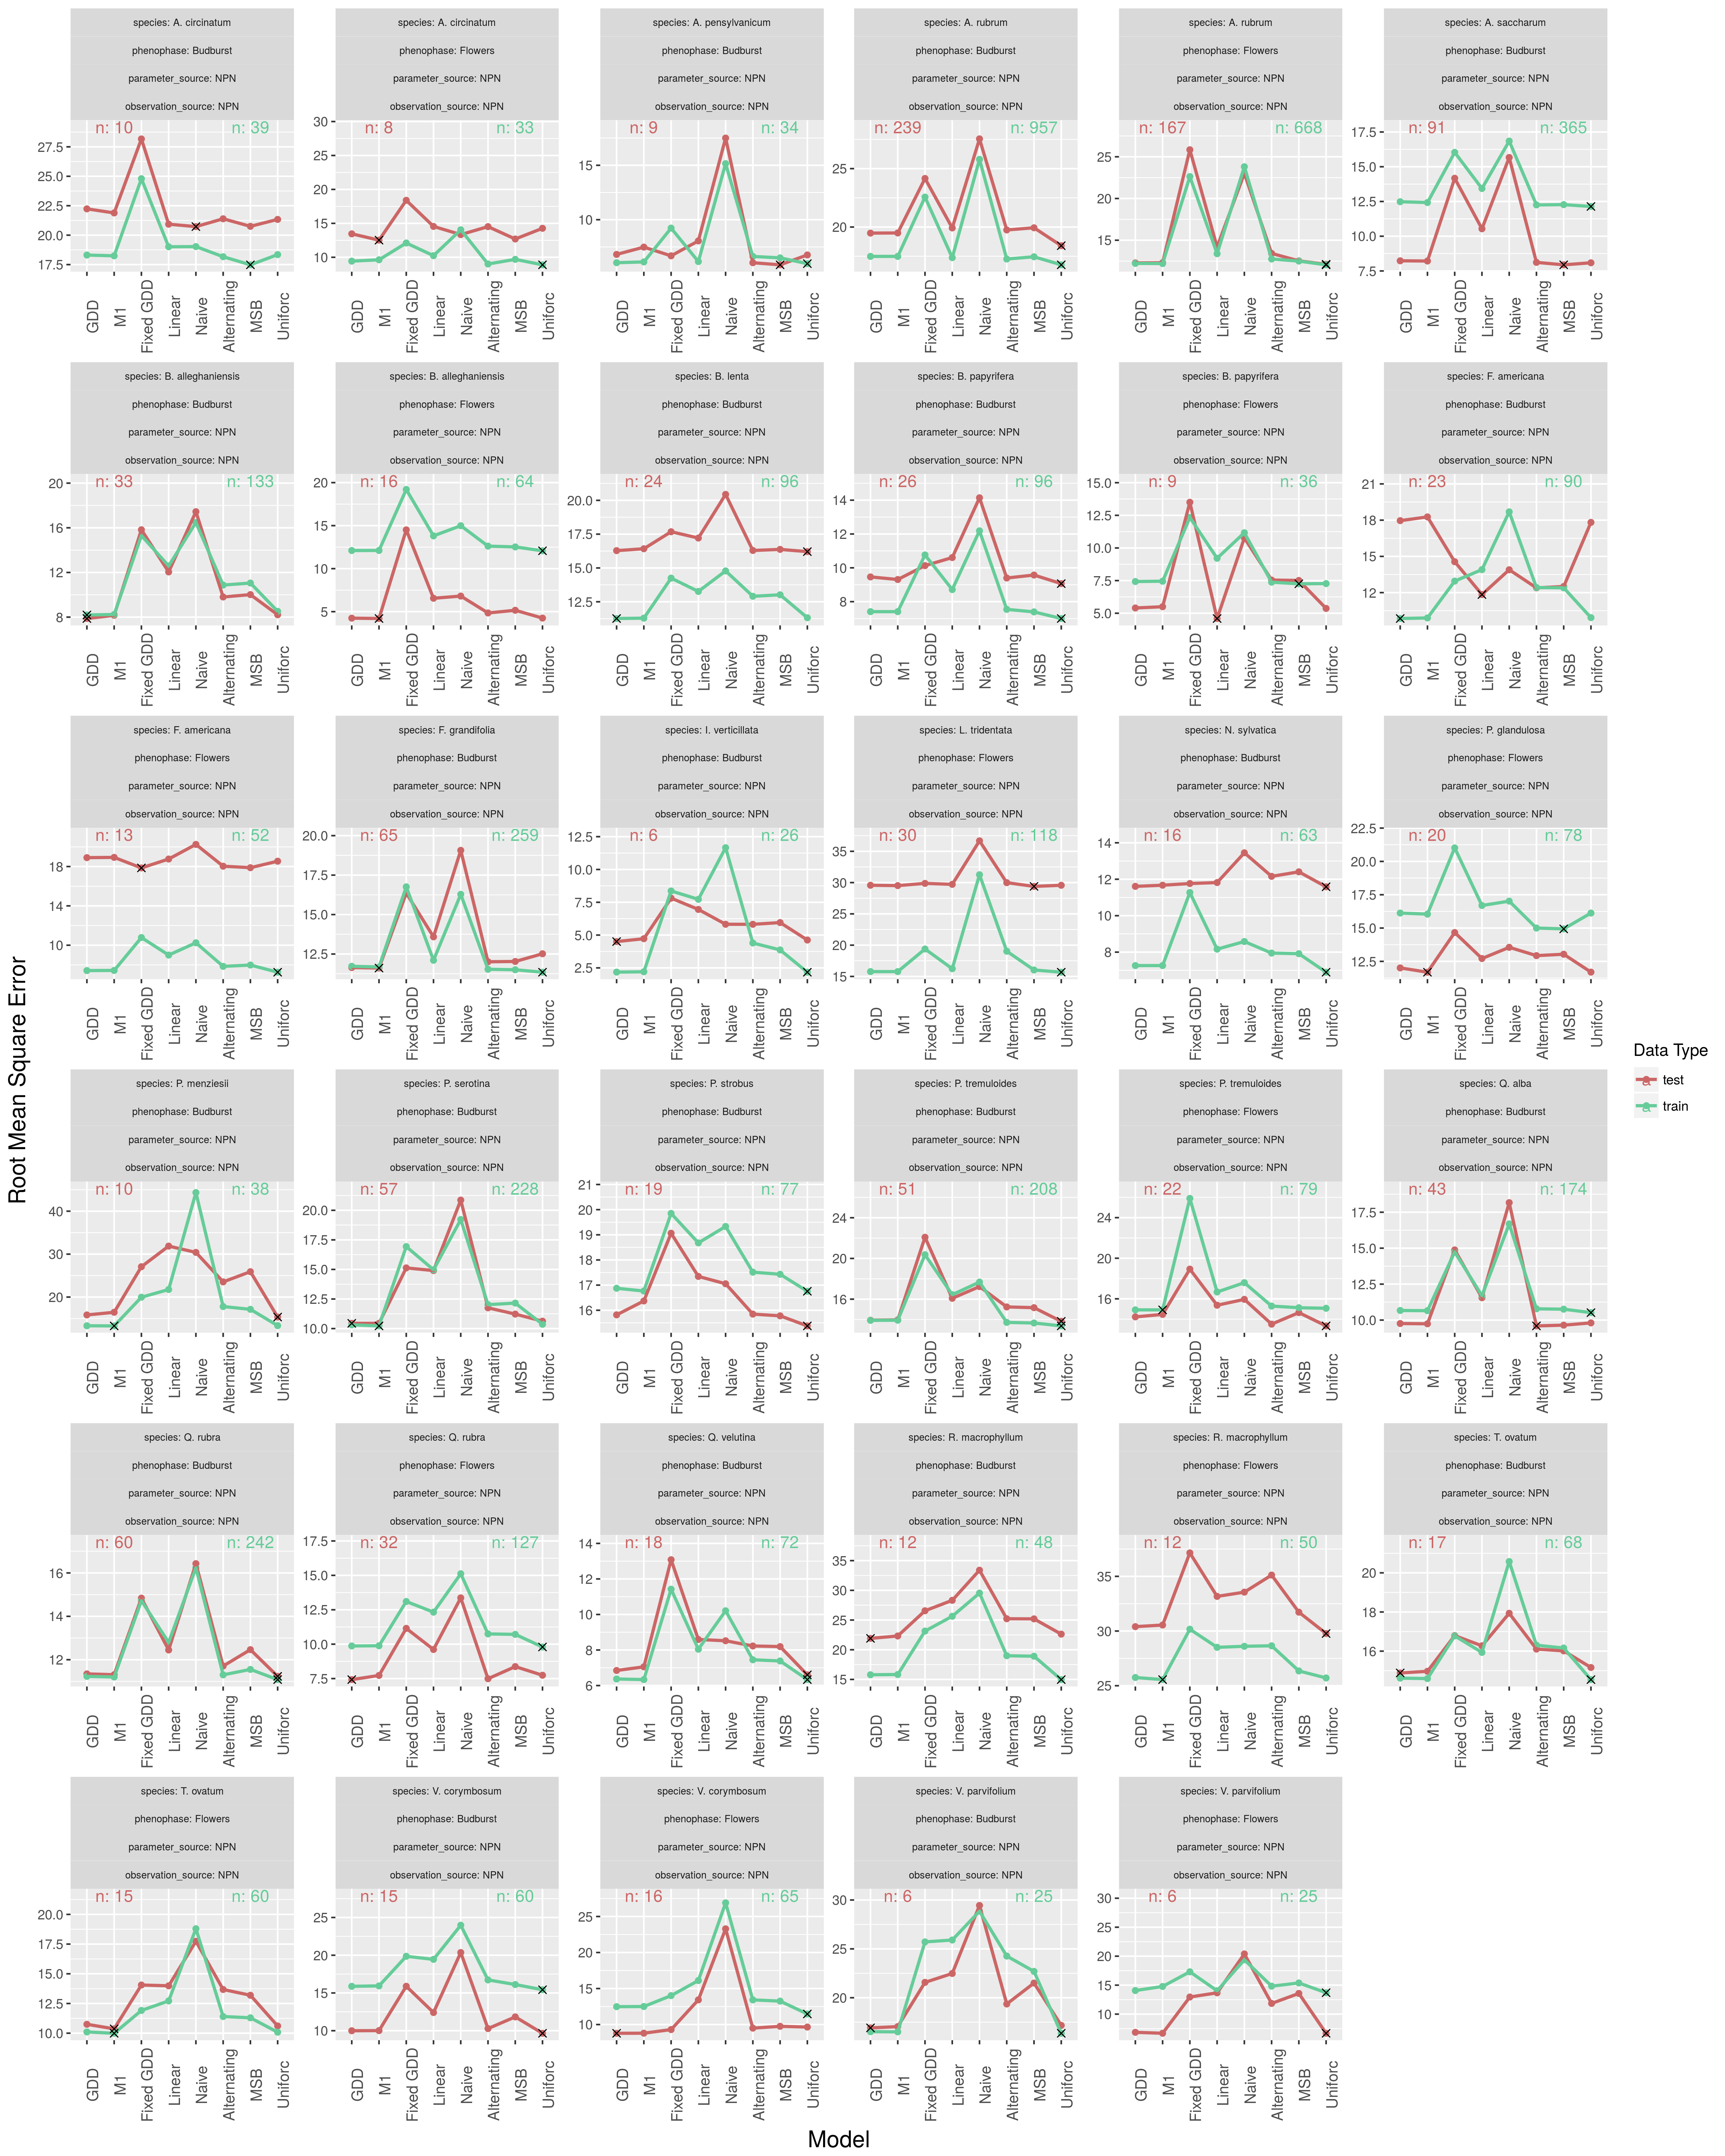
\includegraphics[width=1\textwidth]{supplement_best_npn_models.png}
	\caption{RMSE for specific species and phenophases of the NPN dataset. X marks the best performing models for the respective data type.}
\end{figure}

\begin{figure}
	\centering
		\includegraphics[width=1\textwidth]{supplement_best_lts_models.png}
	\caption{RMSE for specific species and phenophases of the LTS datasets. X marks the best performing models for the respective data type.}
\end{figure}

\begin{figure}
	\centering
		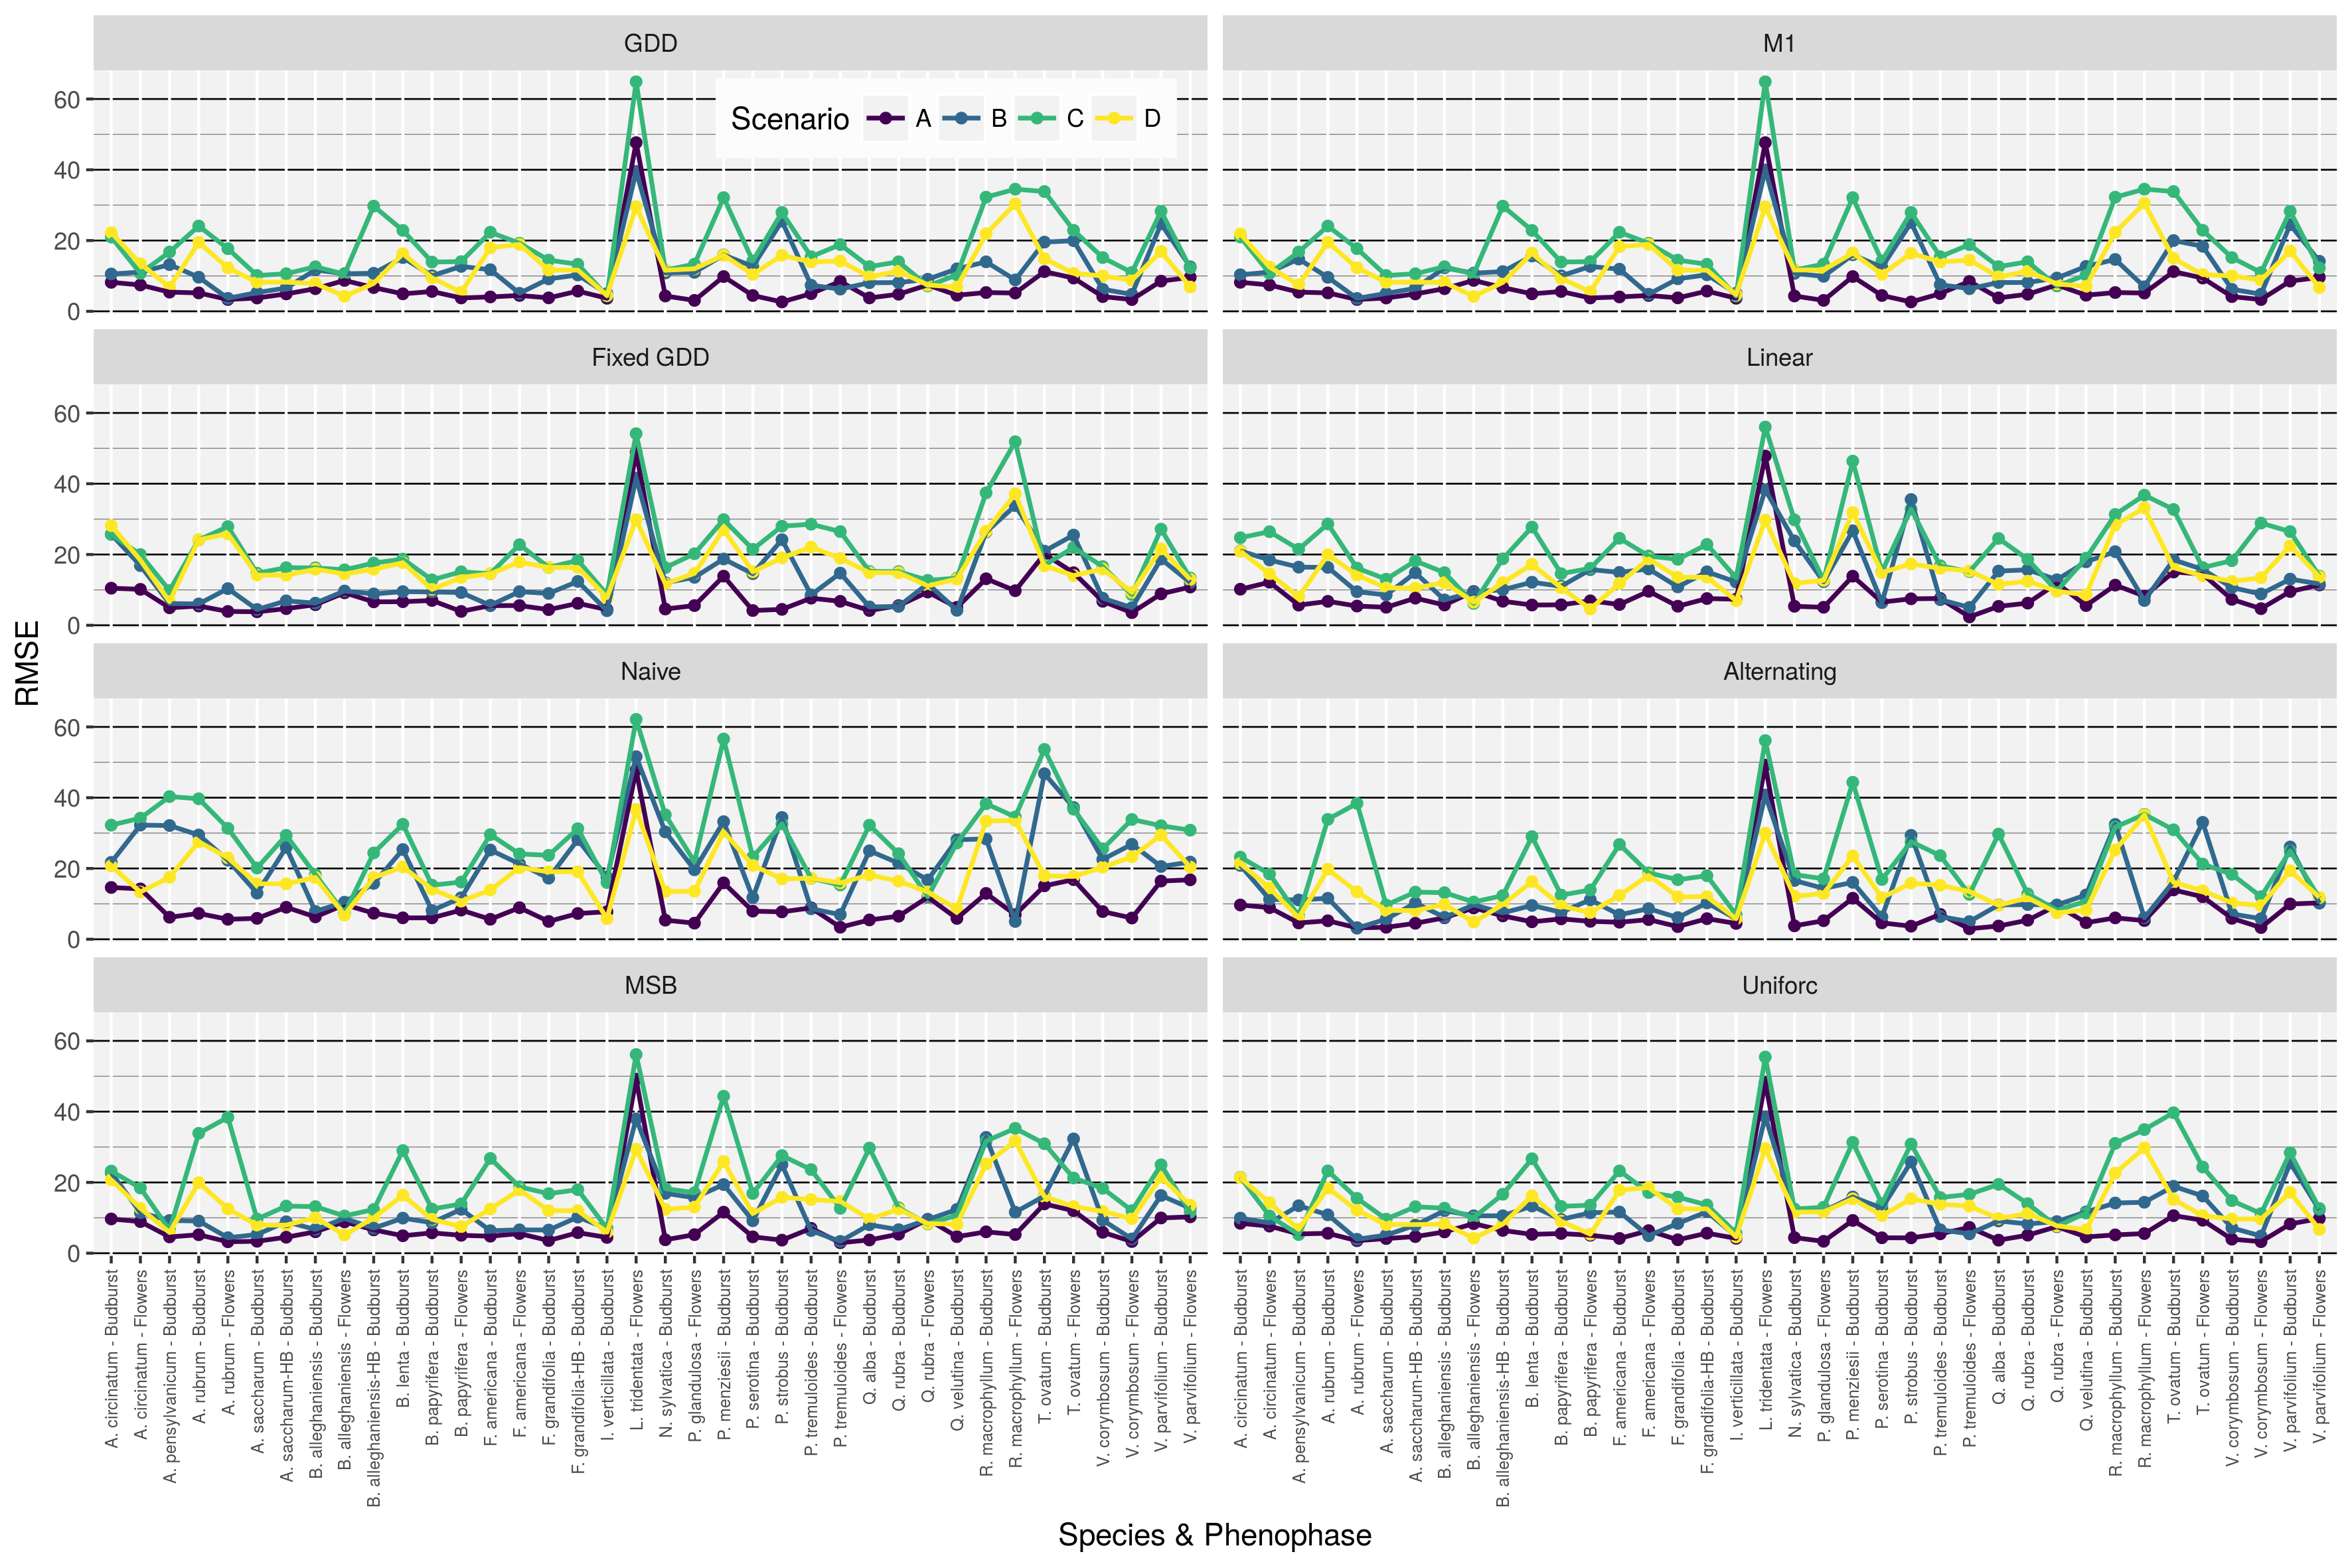
\includegraphics[width=1\textwidth]{supplement_scenario_absolute_rmse.png}
	\caption{RMSE of all species and phenophases of the four scenarios described in the text. These values are calculated using held out test data.}
\end{figure}

\begin{figure}
	\centering
		\includegraphics[width=1\textwidth]{fig_s3_site_map.png}
	\caption{Locations of National Phenology Network sites used (black points) and Long Term Study sites (labeled circles).}
\end{figure}



\end{document}
